\chapter{Discussion}

\section{Photometry}
\label{photo_discussion}

Analysis of the August 2006 data for EC2117 reveals the presence of rapid oscillations. These are limited to DNOs and lpDNOs for the August 2006 dataset. The methods used to find and analyse rapid oscillations are not suitable to find QPOs. This is due to their low coherence and the fact that Fourier methods do not readily reveal the presence of non-stationary signals. More suitable methods do exist \citep{blackman}, but are outside the scope of this project. The lpDNOs do not show any systematic behaviour in the August 2006 photometric runs. They were only present in short sections of the lightcurves and could not be succesfully tracked through eclipse. Their point of origin in the system are therefore still unknown and the models suggested in \cite{DNOQPO_II} and \cite{DNOQPO_VI} cannot be tested using this dataset. 

The DNOs undergo different systematic phase changes through eclipse in multiple lightcurves. In run S7651, during the second eclipse (top-right panel of Fig. \ref{S7651_DNO}, and during the first eclipse of run S7655 (top-left panel of Fig. \ref{S7655_DNO}) it has a phase change similar to that of UX Uma (see Figure 7 in \cite{1980ApJ...241..247P}) where the phase changes by 1 cycle during eclipse. The DNO phase changes by $\sim$1 cycle before changing back to the phase that was present before the eclipse started in the first eclipse of run S7651 and second eclipse of run S7655. The same behaviour is seen in Z Cha during superoutburst in the middle panel of Fig. 10 in \cite{warner_brickhill}. These different scenarios are also encountered in EC2117-54 data retrieved from the archive.  There is also a smaller (shallower, faster) phase change before the aforementioned phase changes. 

The UX Uma-type phase change is explained in \cite{1980ApJ...241..247P} by a rotating-beam model. In this model it is assumed that the disk is axisymmetric; that the oscillation originates from a single spot on the equator of the white dwarf and that some the light from the emission spot is observed directly. The main variable parameter is the inclination of the system which is varied such that the white dwarf is not totally eclipsed. 

\cite{1980ApJ...241..247P} also simulates the phase change during eclipse of the 71s oscillation observed in DQ Her \citep{dqher} using a similar model to that of UX Uma. However, in the DQ Her model, the light from the emission spot is reprocessed and not seen directly. In this model, the phase change during eclipse is sinusoidal and highly dependent on the inclination of the system. Phase changes corresponding to different values for the system inclination are shown in Fig. 4 of \cite{1980ApJ...241..247P}. The sinusoidal curve predicted by the model for the phase change suggests that the Z Cha-type phase changes can be explained to some extent using this model. The idealised model from \cite{1980ApJ...241..247P} could perhaps be used to estimate the orbital inclination, however, this is outside the scope of this project and was not attempted.  The pre-eclipse phase change could possibly be attributed to an obscuration of the DNO source by the disk-stream impact zone, which is almost certainly a thicker region than the rest of the disk and could therefore obscure the white dwarf.

\begin{figure}
 \centering
 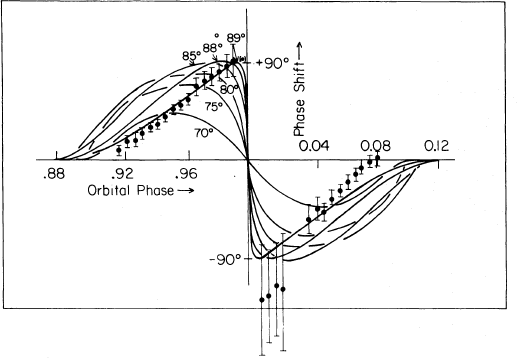
\includegraphics[width=0.75\columnwidth,bb=0 0 517 358]{images/Petterson_Fig4_2.png}
 % Petterson_Fig4.png: 885x446 pixel, 72dpi, 31.22x15.73 cm, bb=0 0 885 446
 \caption[Fig. 4 from \cite{1980ApJ...241..247P}]{Reproduction of Figure 4 from \cite{1980ApJ...241..247P}. The solid lines are models at various inclinations and the points with errorbars are the observations from DQ Her.}
\end{figure}



The fact that EC2117 exhibits two different types of DNO phase changes during eclipse may be explained tentatively by the model given in \cite{1980ApJ...241..247P}, if the possibility is allowed that the emission region on the white dwarf is not always directly visible. This would then imply that it is possible to observe reprocessed light from DNOs. Double DNOs have been observed in EC2117-54 \cite{WWP}. They have also been observed in VW Hyi \citep{warner_ro2004}. It was shown that the DNO with the longer period is the true DNO modulated at the QPO frequency and is therefore light reprocessed off a travelling wave \citep{DNOQPO_II}. Figure 2 of \cite{WWP} displays the periodogram of a section of run S6544 of EC2117-54. A double DNO and an lpDNO peak can be seen. This could explain both types of behaviour and would also support the LIMA model of \cite{DNOQPO_II} in which beamed radiation from the slipping equatorial belt is expected. Clearly the rotating beam model \citep{1980ApJ...241..247P} can be extended to include a concave accretion disk, multiple emission spots, non-axisymmetric accretion disk, visibility of emission regions etc. allowing further investigation into the nature of DNOs.


\section{Spectroscopy}

Analysis of the August 2006 spectroscopic run with SALT did not produce any evidence of rapid oscillations in EC2117-54. The observations were made during the PV phase of SALT, when its instruments were not yet fully operational. The not yet commissioned continuous readout mode would have provided about twice as much data and therefore almost double the signal. This, together with the very low throughput in the blue region of the instrument, made the detection of inherently small variations difficult. Figure \ref{snr} displays the S/N, as a function of orbital phase, of continuum regions in the red, yellow and blue regions of the spectrum. The blue end of the spectra are significantly more noisy than the red end. Because only observations with high S/N (S/N $\geq$ 10) were used to create the phase-folded spectra, the total absence of any detected line modulations at DNO and lpDNO periods suggests that EC2117-54 does not show rapid line modulations. Evidence against this hypothesis is the non-detection of DNOs in lightcurves created from the spectroscopic data even though they are clearly present in simultaneous photometric observations. This suggests that the S/N of the spectroscopic data is too low to detect DNOs at all. At this point it is unclear if emission line modulations from rapid oscillations are expected in EC2117-54. Even though this study did not produce any useful information on the nature of rapid oscillations, future studies of EC2117-54 may be fruitful given the relative high brightness of the object, the expected S/N obtainable with SALT and the regularity with which DNOs are observed in photometric observations.

Because the spectroscopic run was done for only $\sim$40\% of an orbit, robust measurements of the radial velocities and hence the total system mass could not be made. What this spectroscopic run did produce however, is a glimpse of the possibilities of high-speed spectroscopy with SALT. 

\chapter{Conclusions}
A high-speed photometric and spectroscopic study was done on the nova-like cataclysmic variable star EC2117-54. The focus of the study was to learn more about the rapid oscillations that are frequently observed in this object. In particular, the origins of the DNOs and lpDNOs were to be studied by using photometric and spectroscopic observations in combination.
 
The main results of the study are as follows, The Dwarf Nova Oscillations originate on, or very close to, the surface of the primary star; systematic phase changes of the DNO periods during eclipse suggest a rotating beam mechanism for the DNOs.

The spectroscopic run did not produce any evidence of rapid oscillations. The most likely reason for this is the very low signal-to-noise ratio of the observations that was caused by faulty hardware on the telescope during its performance verification phase. Figure \ref{snr} displays signal-to-noise as a function of orbital phase. Faulty optics caused low count rates and hence lower signal-to-noise at the blue end of the spectrum.

The photometric and spectroscopic observations were not fully utilised in this study because it focused only on one aspect of this object. Future studies could use the photometric and spectroscopic data together with additional spectroscopic data in order to have full phase coverage to fully model most system parameters. These would include the masses of the stars, inclination, size of accretion disk, thickness of accretion disk, location of disk-stream impact zone and its size.